% !TeX spellcheck = en_GB
\documentclass[11pt]{article}

\usepackage[type1]{libertine}
\usepackage[a4paper,top=35mm]{geometry}
\usepackage{parskip}
\usepackage{amsmath, amsthm, amssymb} 
\usepackage{booktabs}
\usepackage{tabularx}
\usepackage[english]{babel}
\usepackage{enumitem}	% remove inline if not needed
\usepackage{gensymb}
\usepackage{bm}
\usepackage{graphicx}
\usepackage{xcolor}
\usepackage{float}
\usepackage{wrapfig}
\usepackage[makeroom]{cancel}
\usepackage{multicol}
\usepackage{multirow}
\usepackage{vwcol} 	 	% Provides variable multicol
\usepackage{commath} 	% Provides good differentials
\usepackage{esint} 		% Provides various fancy integral symbols
\usepackage{siunitx} 	% Provides good units
\usepackage{nicefrac}
\usepackage{dashrule}

\usepackage[titletoc,title,toc,page]{appendix}

\newcommand{\nocontentsline}[3]{}
\newcommand{\tocless}[2]{\bgroup\let\addcontentsline=\nocontentsline#1{#2}\egroup}
\newcommand{\stoptocwriting}{%
	\addtocontents{toc}{\protect\setcounter{tocdepth}{-5}}}
\newcommand{\resumetocwriting}{%
	\addtocontents{toc}{\protect\setcounter{tocdepth}{\arabic{tocdepth}}}}

\renewcommand\thetable{\thesection-\arabic{table}}
\renewcommand\thefigure{\thesection-\arabic{figure}}

\usepackage{framed}
\colorlet{shadecolor}{yellow!35!} %BurntOrange!40 yellow!35! Black!20!

% https://tex.stackexchange.com/a/124390
\makeatletter
\renewcommand{\boxed}[2][\fboxsep]{{%
		\setlength{\fboxsep}{#1}\fbox{\m@th$\displaystyle#2$}}}
\makeatother

\usepackage{chngcntr}
\counterwithin{figure}{section}
\numberwithin{equation}{section}

\usepackage{hyperref}
\hypersetup{
	pdftitle={SJPO Training -- Summary of Topics},
	pdfauthor={Lor Jun Heng, Sun Yudong},
	bookmarksnumbered=true,
	bookmarksopen=true,
	bookmarksopenlevel=2,
	pdfstartview=Fit,
	pdfpagemode=UseOutlines,
	colorlinks=true,
	linkcolor=black,
	filecolor=magenta,      
	urlcolor=blue
}
\urlstyle{same}

% custom environments
\newcommand{\uvec}[1]{\boldsymbol{\hat{\textbf{#1}}}}
\newcommand{\bvec}[1]{\boldsymbol{\vec{#1}}}
\def\doubleunderline#1{\underline{\underline{#1}}}

\renewcommand{\ttdefault}{cmtt}

\newenvironment{multicolFigure}
{\par\medskip\noindent\minipage{\linewidth}}
{\endminipage\par\medskip}

\usepackage{titlesec}
%\definecolor{blu}{HTML}{0099CC}
%\newcommand\crule[3][black]{\textcolor{#1}{\rule{#2}{#3}}}
\titleformat{\subsection}[hang]
	{\bfseries}
	{\fbox{\thesubsection}}
	{1em}
	{}
	
\usepackage{fancyhdr}
\pagestyle{fancy}
\fancyhf{}
\lhead{SJPO 2018 Summary of Topics}
\rhead{Prepared by Lor Jun Heng, Sun Yudong}
\cfoot{\thepage}
%\\{\scriptsize Prepared by Lor Jun Heng, Sun Yudong 2018}

\title{SJPO Training 2018\\-- Summary of Topics --}
\author{Lor Jun Heng, Sun Yudong\\Hwa Chong Institution}
\date{May 7, 2018}
	
\begin{document}
\maketitle
The following summary is based on the SJPO 2018 Syllabus. Not all bullet points in the syllabus have been elaborated upon. The complete syllabus has been uploaded onto Google Drive. 
\vfill
\begin{center}
	Good luck\\[0.4em]
	{\Large Don't Panic}
\end{center}
\vspace{3em}
\tableofcontents
\pagebreak
	\section{Mechanics of Particles}
		\subsection{Kinematics {\small \normalfont -- position, displacement, velocity, acceleration, vectors}}
			\begin{center}
				\renewcommand{\arraystretch}{1.5}
				\begin{tabular}[h]{@{}l@{\hspace{2em}}lll@{}}
					\toprule
					Position	&\multicolumn{3}{l}{Position is described by displacement vector $\bvec{x}$ from a fixed point, origin}\\[0.5em]
					Velocity	&$\bvec{v}=\dod{\bvec{x}}{t}$\hspace{3cm} &
					Acceleration&$\bvec{a}=\dod{\bvec{v}}{t}$ \\[0.7em]
					\bottomrule
				\end{tabular}
			\end{center}
			%\vfill
			\subsubsection{Motion of point mass}
				When considering translational motion, we can consider all forces acting on an object to be acting through its centre of mass.
			%\vfill
			\subsubsection{Motion in 1-dimension}
				These equations are derived by integrating a constant acceleration, $a$, using the limits where $t_i=0$, $t_{\!f}=t$, $v_i=u$, $v_{\!f}=v$. Clearly define the coordinate system ie which direction is positive before use.
				\vspace{1em}
				\hrule
				\vspace{-0.7em}
				\begin{align*}
					s=ut+\frac{1}{2}at^2 && v^2=u^2+2as && v=u+at
				\end{align*}
				\hrule
			%\vfill
			\subsubsection{Motion in 2-dimension}
				Motion in more than one dimension can be uniquely separated into its dimensions as long as they are orthogonal (perpendicular) to one another. Each dimension has its own set of independent kinematic equations.
			%\vfill
			\subsubsection{Vector description of motion of a point mass}
				The motion of a point mass can be uniquely defined when its position and momentum (velocity) is known.
			\subsubsection{Relative velocity}
				In an inertial frame travelling at $\bvec{v}_1$ relative to a rest frame, the velocity of an object travelling at $\bvec{v}_2$ in the rest frame appears to be $$\bvec{v}_{\text{apparent}}=\bvec{v}_2-\bvec{v}_1$$
			\subsubsection{Motion with constant acceleration {\small \normalfont \em (e.g. free fall, projectile motion)} or with variable acceleration {\small \normalfont \em (e.g. car on straight road)}}
				Motion with constant acceleration is parabolic/quadratic.
				
				Consider graphical methods when the velocity of an object changes multiple times in a question.
				
				A general rule-of-thumb of integration is that any \textbf{polynomial} function, when integrated, will have its power increased by 1. $\left(\text{e.g. } x^2 \rightarrow x^3\right)$.\footnote{Note that this does not apply to $\int\frac{1}{x}=\ln x + C$} Similarly, any \textbf{polynomial} function, when differentiated, will have its power decreased by 1. $\left(\text{e.g. } x^3 \rightarrow x^2\right)$.
			\subsubsection{Motion in a circle {\small \normalfont \em (involving centripetal acceleration)}}
				For an object to undergo circular motion, the net force acting on the object must be
				\begin{equation*}
					\bvec{F}_{\text{net}} = m\bvec{a}_{\text{centripetal}} = m\frac{v^2}{r} = mr\omega^2
				\end{equation*}
				in the radial direction.
				
				\textbf{Note:} Centripetal force isn't a physical force, rather it is a condition for the net force acting on an object that is undergoing circular motion.
		%\vfill
		%\pagebreak
		\subsection{Dynamics {\small \normalfont -- inertia, momentum, impulse, forces, energy}}
			\begin{center}
				\renewcommand{\arraystretch}{1.5}
				\begin{tabular}[h]{@{}l@{\hspace{2em}}p{11cm}@{}}
					\toprule
					Inertia	&A property of matter by which it continues in its existing state of rest or uniform motion in a straight line, unless that state is changed by an external force. Related to the mass of an object \\[0.5em]
					Impulse	&$\bvec{J}=\Delta \bvec{P}=\bvec{F}_{\text{avg}} \Delta t=m \Delta\bvec{v}$ \\[0.7em]
					Forces&$\bvec{F}=\dod{\bvec{p}}{t} = m\dod{\bvec{v}}{t}$ (for constant mass) aka Newton’s second law \\[0.5em]
					&$\displaystyle \bvec{F}_{\text{avg}} = m \bvec{a}_{\text{avg}} = m \frac{\Delta v}{\Delta t}$ \\[0.5em]
					\bottomrule
				\end{tabular}
			\end{center}
			\vfill
			\pagebreak
			\subsubsection{Newton’s laws of motion/Application of Newton’s laws}
				Newton's first law states that every object will remain at rest or in uniform motion in a straight line unless compelled to change its state by the action of an external force. This is normally taken as the definition of inertia. The key point here is that if there is no net force acting on an object (if all the external forces cancel each other out) then the object will maintain a constant velocity. If that velocity is zero, then the object remains at rest. If an external force is applied, the velocity will change because of the force.
				
				The second law explains how the velocity of an object changes when it is subjected to an external force. The law defines a force to be equal to change in momentum (mass $\times$ velocity) per change in time. Newton also developed the calculus of mathematics, and the ``changes" expressed in the second law are most accurately defined in differential forms. (Calculus can also be used to determine the velocity and location variations experienced by an object subjected to an external force.) For an object with a constant mass $m$, the second law states that the force $\bvec{F}$ is the product of an object's mass and its acceleration $\bvec{a}$:
				\begin{equation*}
					\bvec{F}=m\bvec{a}
				\end{equation*}
				For an external applied force, the change in velocity depends on the mass of the object. A force will cause a change in velocity; and likewise, a change in velocity will generate a force. The equation works both ways.
				
				The third law states that for every action (force) in nature there is an equal and opposite reaction. In other words, if object $A$ exerts a force on object $B$, then object $B$ also exerts an equal force on object $A$. Notice that the forces are exerted on different objects. The third law can be used to explain the generation of lift by a wing and the production of thrust by a \textbf{jet engine}.
				
				\url{https://www.grc.nasa.gov/www/k-12/airplane/newton.html}
			\subsubsection{Motion affected by dissipative forces {\small \normalfont \em (e.g. friction, fluid resistance)}}
				Kinetic friction is constant and acts in the opposite direction of motion $F_{\text{kinetic}} = \mu_k N$.
				
				Other kinds of resistance are proportional to the $v$ or $v^2$ of the object and act in the opposing direction. The resultant motion is exponential decay for the former while the latter is similar in shape but has a sharper decrease.
			%\pagebreak
			\subsubsection{Elastic, friction, normal, gravity including Newton’s law of gravitation, electric and magnetic}
				\begin{center}
					\renewcommand{\arraystretch}{1.5}
					\begin{tabular}[h]{@{}l@{\hspace{2em}}p{9.5cm}@{}}
						\toprule
						Elastic Force	& $F_{\text{elastic}} = -kx$\\
						\multirow{2}{*}{Friction} & $f_{\text{static}} \leq \mu_sN$ \\
						& $f_{\text{kinetic}} = \mu_kN$ \\
						Normal Contact Force & Normal force occurs between two surfaces and is perpendicular to the surface \\
						\multirow{2}{*}{Gravity} & $F_g = mg$ near surface of Earth \\[0.5em]
						& $\displaystyle F = \frac{GMm}{r^2}$ towards each other \\[0.7em]
						Coloumb's law & $\displaystyle \frac{1}{4\pi\varepsilon_0}\cdot \frac{q_1q_2}{r^2}$ \\[0.5em]
						Force by an electric field & $\bvec{F}_{\boldsymbol{\!E}} = q\bvec{E}$ \\
						Magnetic Force & $\bvec{F}_{\boldsymbol{\!B}} = q\bvec{v}\times\bvec{B}$ \\[0.3em]
						\bottomrule
					\end{tabular}
				\end{center}
		%\pagebreak
		\subsection{Conservation of energy, conversion of energy}
			Energy is always conserved in a closed system in an inertial frame. Energy can be converted to other forms by cannot be destroyed.
			\subsubsection{Work Done, Power, Potential Energy (PE), Kinetic Energy (KE)}
				\begin{center}
					\renewcommand{\arraystretch}{1.5}
					\begin{tabular}[h]{@{}l@{\hspace{2em}}p{9cm}@{}}
						\toprule
						Work Done & $W = \bvec{F}\cdot \bvec{d}~$ Work done by an object through a force is equal to the product of the magnitude of the force acting parallel to the direction of motion.
						\\
						Power & $P = \dod{W}{t}$ \\[0.5em]
						Elastic PE	& $\text{EPE} = \frac{1}{2}kx^2$\\
						Work done against Friction & $W_{\!f} = \bvec{f} \cdot \bvec{d}$ \\
						\multirow{2}{*}{Gravitational PE} & $\text{GPE}= mgh~~$ (for small values of h at the surface of earth)\\[0.5em]
						& $\displaystyle \text{GPE} = -\frac{GMm}{r}~~$ (in general)\\[0.5em]
						\multirow{2}{*}{Electric PE} & $\displaystyle \text{EPE} = q \Delta V = q \int_{r_0}^{r_1} e \dif r$ \\[0.7em]
						&$\displaystyle \text{EPE} = \frac{1}{4\pi\varepsilon_0}\cdot\frac{q_1q_2}{r}~~$ for two particles in free space\\[0.5em]
						Kinetic Energy & $\text{KE}=\frac{1}{2}mv^2$ \\[0.5em]
						\bottomrule
					\end{tabular}
				\end{center}
		%\pagebreak
		\subsection{Impulse and Momentum / Conservation of Linear Momentum}
			Momentum $\bvec{p}=m\bvec{v}$ is conserved in any closed system due to newton’s third law.
			\subsubsection{Collisions/explosions}
				There are two types of collisions: Inelastic and elastic. For elastic collisions, both energy and momentum is conserved. This leads to the condition that the velocity of approach must be equal and in opposite direction to the receding velocity:
				\begin{equation*}
					u_1-u_2=-(v_1-v_2)
				\end{equation*}
			\pagebreak
			\subsubsection{Coefficient of Restitution}
				$e$ is the ratio of the final to initial relative velocity between two objects after they collide, usually a positive, real number between 0 and 1:
				\vspace{1em}
				\begin{center}
					\renewcommand{\arraystretch}{1.5}
					\begin{tabular}[h]{@{}l@{\hspace{2em}}p{12cm}@{}}
						\toprule
						$e=0$ & This is a perfectly inelastic collision. The objects do not move apart after the collision, but instead they coalesce. Kinetic energy is converted to heat or work done in deforming the objects. \\
						$0 < e < 1$ & This is a real-world inelastic collision, in which some kinetic energy is dissipated. \\
						$e = 1$ & This is a perfectly elastic collision, in which no kinetic energy is dissipated, and the objects rebound from one another with the same relative speed with which they approached. \\
						\toprule
					\end{tabular}
				\end{center}
				\vspace{1em}
			\subsubsection{External and internal forces for a system of particles, centre of mass}
				Internal forces cannot be detected from outside the system. They do not cause a change in total momentum or energy of a system. The resultant force of an internal force acts on another object in the system.
				
				External forces causes a change in the total momentum and energy of a system and its resultant force acts on an object outside the system.
				
				COM is the weighted average of the displacement of the masses
				\begin{equation*}
					x_{\text{COM}}= \frac{1}{M} \sum_{i} m_ir_i \text{~~where~~} M = \sum_{i} m_i
				\end{equation*}
				For continuous distribution:
				\begin{equation*}
					x_{\text{COM}}= \frac{1}{M} \int r \dif m
				\end{equation*}
	\section{Mechanics of Rigid Bodies}
		\subsection{Statics {\small \normalfont -- equilibrium, stability}}		
			\begin{center}
				\renewcommand{\arraystretch}{1.5}
				\begin{tabular}[h]{@{}l@{\hspace{2em}}p{9.5cm}@{}}
					\toprule
					\textbf{Static equilibrium} & is attained when the net forces acting on an object is zero. \\
					\textbf{Rotational equilibrium} & is attained when the net torque acting on an object is zero. \\
					\textbf{Stable equilibrium} & is attained when a small disturbance from its position is met with a restoring force. \\
					\textbf{Dynamic equilibrium} & is attained when a small disturbance from its position causes a net force acting in the same direction. \\
					\textbf{Neutral equilibrium} &is attained when the system experiences not net force after a small disturbance. \\
					\bottomrule
				\end{tabular}
			\end{center}
		\subsection{Kinematics {\small \normalfont -- angular position, angular displacement, angular velocity, angular acceleration, vector products}}
			\begin{center}
				\renewcommand{\arraystretch}{1.5}
				\begin{tabular}[h]{@{}l@{\hspace{2em}}p{10cm}@{}}
					\toprule
					$\theta$ & Angular displacement relative to an angle \\[0.5em]
					Angular Velocity & $\bvec{\omega} = \dod{\bvec{\theta}}{t}$ \\[1em]
					Angular acceleration & $\bvec{\alpha} = \dod{\bvec{\omega}}{t}$ \\[0.7em]
					\bottomrule
				\end{tabular}
			\end{center}
			\vspace{1em}
			The direction of angular displacement/velocity/acceleration is given by the right-hand-rule.
			\subsubsection{Rotation with constant angular acceleration}
				Akin to kinematic equations:
				\vspace{1em}
				\hrule
				\vspace{-1em}
				\begin{align*}
					\text{Moment of Inertia}&& I&=\int r^2 \dif m \\
					\text{Displacement} && \theta&=\omega t + \frac{1}{2}\alpha t^2 \\
					\text{Velocity} && \omega_f^2 &=\omega_i^2 + 2\alpha\theta\\
					\vdots && \vdots
				\end{align*}
				\vspace{-0.5em}
				\hrule
			\pagebreak
			\subsubsection{Relationship between linear and angular quantities}
				\begin{equation*}
					\boxed[2\fboxsep]{\bvec{v} = \bvec{r} \times \bvec{\omega}}
					~~~~~~~~~~~~~~~~~~~~~~~~~~
					\boxed[2\fboxsep]{\bvec{a} = \bvec{r} \times \bvec{\alpha}}
				\end{equation*}
		\subsection{Dynamics {\small \normalfont -- moment of inertia, torque}}
			\begin{equation*}
				\boxed[2\fboxsep]{\bvec{\tau} = I\bvec{\alpha} = \bvec{r}\times\bvec{F}}
			\end{equation*}
			\subsubsection{Angular momentum}
				\begin{equation*}
					\boxed[2\fboxsep]{\bvec{L}=\bvec{r}\times \bvec{p}=mvr\sin\theta ~\uvec{n}}
				\end{equation*}
				Angular motion is conserved in a closed system. It remains constant if no torque is acting upon the body.
				
				For circular motion, $L=mvr$.
			\subsubsection{Rotational KE}
				\begin{equation*}
					\boxed[2\fboxsep]{\text{Rotational KE}=\frac{1}{2}I\omega^2}
				\end{equation*}
	\pagebreak
	\section{Fluid Mechanics}
		\subsection{Fluid statics {\small \normalfont -- Density, pressure, buoyancy, surface tension}}
			\begin{center}
				\renewcommand{\arraystretch}{2}
				\begin{tabular}[h]{@{}l@{\hspace{2em}}p{10cm}@{}}
					\toprule
					\textbf{Pressure} & $\displaystyle P=\frac{F}{A} = \rho g h \text{~in a fluid} \hfill \text{where~} \rho=\frac{M}{V} \hfill$\\[0.7em]
					\textbf{Buoyancy Force} & Buoyancy force is equal to the weight of fluid displaced caused due to difference of pressure between the top and body of an object. \\
					\textbf{Surface tension} & $\sigma = \gamma l$ where $\gamma$ is a constant based on the property of the fluid and l is the length of surface exposed to the liquid. For a film, the total surface tension is double since there are two surfaces. \\
					\bottomrule
				\end{tabular}
			\end{center}
			\subsubsection{Pascal's law, Archimedes' principle}
				\begin{center}
					\renewcommand{\arraystretch}{2}
					\begin{tabular}[h]{@{}l@{\hspace{2em}}p{10cm}@{}}
						\toprule
						\textbf{Pascal's Law} & Pascal's law (also Pascal's principle or the principle of transmission of fluid-pressure) is a principle in fluid mechanics that states that a pressure change occurring anywhere in a confined incompressible fluid is transmitted throughout the fluid such that the same change occurs everywhere. (i.e the pressure of a fluid at a height is always equal.) \\
						\textbf{Archimedes' principle} & Archimedes' principle states that the upward buoyant force that is exerted on a body immersed in a fluid, whether fully or partially submerged, is equal to the weight of the fluid that the body displaces and acts in the upward direction at the center of mass of the displaced fluid. $$F_u = \rho V_{\text{displaced}} g = \rho V\!g$$ \vspace{-1em}\\
						\bottomrule
					\end{tabular}
				\end{center}
		\pagebreak
		\subsection{Fluid Dynamics}
			\subsubsection{Bernoulli’s principle}
				\textbf{Bernoulli's principle} states that an increase in the speed of a fluid occurs simultaneously with a decrease in pressure or a decrease in the fluid's potential energy. 
				\begin{equation*}
					\frac{v^{2}}{2}+gz+\frac{p}{\rho}=\text{constant}
				\end{equation*}
				where:
				\begin{enumerate}[label={}]
					\item $v =$ Fluid flow speed at a point on a streamline
					\item $g =$ Acceleration due to gravity
					\item $z =$ Elevation of the point above a reference plane, with the positive $z$-direction pointing upward – so in the direction opposite to the gravitational acceleration
					\item $p = $ Pressure at the chosen point
					\item $\rho = $ Density of the fluid at all points in the fluid
				\end{enumerate}
				The following assumptions must be met for this Bernoulli equation to apply:
				\begin{itemize}
					\item the flow must be steady, i.e. the flow parameters (velocity, density, etc...) at any point cannot change with time
					\item the flow must be incompressible – even though pressure varies, the density must remain constant along a streamline
					\item friction by viscous forces must be negligible
				\end{itemize}
	\pagebreak
	\section{Oscillations and Waves}
		\subsection{Simple Harmonic Motion}
		The general form of a SHM is as follows:
		\begin{equation*}
			A=A_0\sin(\omega t+\phi)
		\end{equation*}
		Solution of the SHM equation:
		\begin{equation*}
			\bvec{a}=-k\bvec{x} ~~~~~~~~~ \text{~~where~~} k=\omega^2=\left(\frac{2\pi}{T}\right)^2
			\vspace{-1em}
		\end{equation*}
		
		\subsection{Mechanical, Electrical}
			\subsubsection{Frequency, Period, Phase Difference}
				\begin{center}
					\renewcommand{\arraystretch}{1.5}
					\begin{tabular}[h]{@{}l@{\hspace{2em}}p{10cm}@{}}
						\toprule
						Frequency $f$ & Number of oscillations that occur per second \\
						Period $T$ & Time taken for an oscillation to occur, the inverse of frequency \\
						Phase Difference $\Delta\phi$ & The difference in the phase angle between two oscillating systems ie how much one system is leading another \\
						& If they are in phase, the phase difference is equal to $2\pi$ and the two systems reach their maxima and minima at the same time. \\
						& If they are out of phase, the phase difference is $\pi$ and the maxima of one system occurs at the minima of another system. \\
						\bottomrule
					\end{tabular}
				\end{center}
			\subsubsection{Qualitative understanding of damping and resonance}
				\textbf{Damping} occurs when a force opposes a system’s change, it is modelled as proportional to the system’s rate of change i.e drag force. There are three types of damping: 
				\begin{center}
					\renewcommand{\arraystretch}{1.5}
					\begin{tabular}[h]{@{}l@{\hspace{2em}}p{8cm}@{}}
						\toprule
						\multirow{3}{6cm}{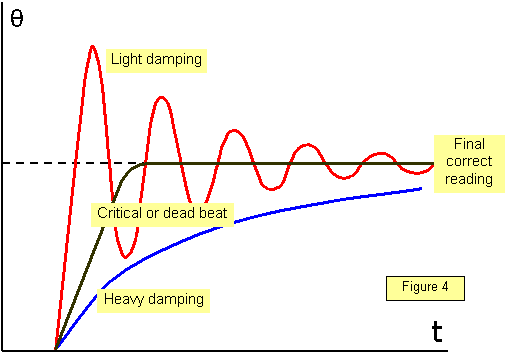
\includegraphics[width=6cm]{damping.png}}& \textbf{Lightly Damped}\par Still sinusoidal but the amplitude is contained in an exponential decay envelope. \\
						&\textbf{Overdamped} \par Never passes the origin, tends towards equilibrium \\
						&\textbf{Critically Damped} \par May pass through the origin at most once. Reaches the origin in the fastest possible time.\\
						\bottomrule
					\end{tabular}
				\end{center}
		\pagebreak
		\subsection{Waves: Mechanical {\small \normalfont \em (Sound, String, Fluid)}, Electromagnetic}
			For a wave traveling in the positive $x,~k>0$, it has a general equation:
			\begin{equation*}
				y = A\sin(\omega t-kx+\phi)
				\vspace{-1em}
			\end{equation*}
			\begin{center}
				\renewcommand{\arraystretch}{1.5}
				\begin{tabular}[h]{@{}l@{\hspace{2em}}p{10cm}@{}}
					\toprule
					Attenuation & The loss of energy of a wave over a distance. \\
					Wavelength $\lambda$ & The distance of space over which a wave repeats \\
					Wave Speed $v$ & The speed at which a wave propagates. $v = f\!\lambda$ \\
					Amplitude $A$, Intensity $I$ & $I \propto A^2$\\
					Transverse Waves & Transverse waves oscillate in the plane \textbf{perpendicular} to the direction of propagation. \\
					Longitudinal Waves & Longitudinal waves oscillate \textbf{along} the direction of propagation.\\
					\bottomrule
				\end{tabular}
			\end{center}
			\subsubsection{Polarization, Malus’ law}
				Polarized light occurs when the vibrations only occur along a single plane.
				
				Malus' law states that the intensity of a beam of plane-polarized light after passing through a rotatable polarizer varies as the square of the cosine of the angle through which the polarizer is rotated from the position that gives maximum intensity:
				\begin{equation*}
					I=I_0\cos^2\theta \impliedby A=A_0\cos\theta
				\end{equation*}
				\begin{center}
					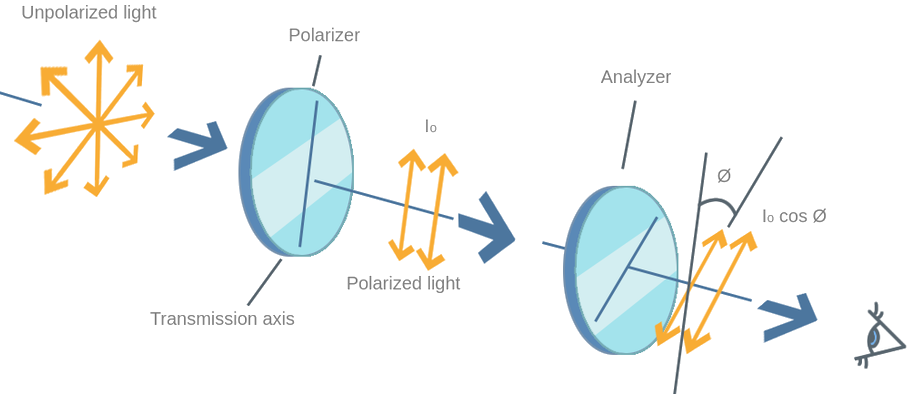
\includegraphics[height=5cm]{maluslaw.png}
				\end{center}
			\subsubsection{Principle of superposition}
				The net displacement of the sum of waves at a point is equal to the sum of the displacements caused by each wave separately. (i.e. waves can be added on each other)
			\subsubsection{Standing waves, interference, diffraction, beats}
				\begin{center}
					\renewcommand{\arraystretch}{1.5}
					\begin{tabular}[h]{@{}l@{\hspace{2em}}p{10cm}@{}}
						\toprule
						Standing waves & Standing waves occur when two waves travelling in opposite directions interfere and form a wave where the nodes and antinodes have fixed positions. \\
						Interference & Interference occurs when two waves in the same medium superpose. \\
						&Constructive interference occurs when the waves are in phase. \\
						& Destructive interference occurs when the waves are exactly out of phase.\\
						Diffraction & Diffraction occurs when waves bend around corners of an object or aperture into the geometrical shadow of the obstacle. \\
						Beats & Beats occur when two waves interfere. It results in a sinusoidal pattern where the amplitude is controlled by another sinusoidal pattern.
						\vspace{1.5em}
						\begin{center}
							\vspace{-0.3cm}
							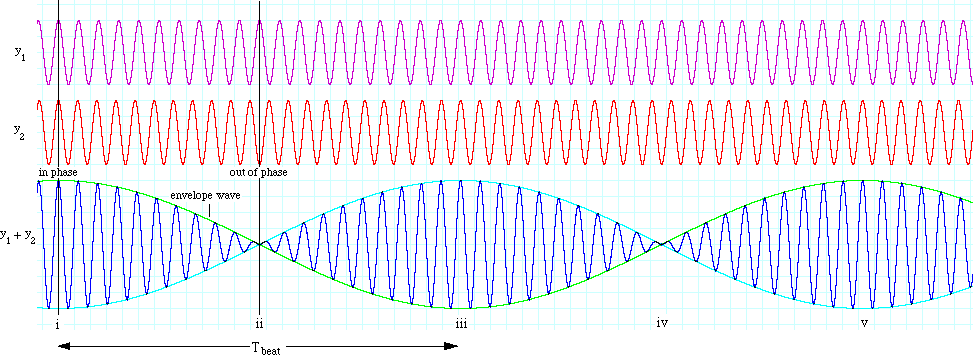
\includegraphics[width=10cm]{beats.png}
							\vspace{-0.8cm}
						\end{center} 
						\\
						\bottomrule
					\end{tabular}
				\end{center}
				More at \url{http://www.physicsclassroom.com/class/sound/Lesson-3/Interference-and-Beats}.
		\subsection{Geometric Optics}
			\begin{center}
				\renewcommand{\arraystretch}{1.5}
				\begin{tabular}[h]{@{}l@{\hspace{2em}}p{10cm}@{}}
					\toprule
					Reflection& $\theta_\text{incident} = \theta_\text{reflected}$ \\
					Refraction& Optical Density of medium $\displaystyle \eta = \frac{c}{v_{\text{light in medium}}}$
					\begin{equation*}
						\frac{\sin\theta_i}{\sin\theta_r} = \frac{\eta_i}{\eta_r}
					\end{equation*}
					Refer to {\small \url{hyperphysics.phy-astr.gsu.edu/hbase/Tables/indrf.html}} for common refractive indices.\\
					Total Internal Reflection & From medium with greater optical density to a lower one:
					\begin{equation*}
						\theta_i > \theta_c \text{~~where~~} \frac{1}{\sin \theta_c} =  \frac{\eta_i}{\eta_r}
						\vspace{-1em}
					\end{equation*}
					\\
					\bottomrule
				\end{tabular}
			\end{center}
	\section{Electric Charge and Electric Field}
		\begin{center}
			\renewcommand{\arraystretch}{2}
			\begin{tabular}[h]{@{}l@{\hspace{2em}}l@{}}
				\toprule
				Coulomb's Law & $\displaystyle \frac{1}{4\pi\varepsilon_0} \cdot \frac{q_1q_2}{r^2}$\\[0.5em]
				Electric Field & $\displaystyle E = \frac{1}{4\pi\varepsilon_0} \cdot \frac{\sum_i q_i}{r^2} = \frac{1}{4\pi\varepsilon_0} \sum \frac{\dif q}{r^2}$ \\[0.5em]
				Electric Flux & \multirow{2}{*}{$\displaystyle \Phi = \int\! \bvec{E}\cdot \dif\bvec{A} = \bvec{E}\cdot \bvec{A}$} \\
				\hspace{2em}\begin{minipage}{7.5cm}
					$ \Rightarrow $ Analogous to the number of field lines cutting through a surface per area
				\end{minipage} & \\
				Electric Potential & $\displaystyle V = \frac{1}{4\pi\varepsilon_0} \cdot \frac{\sum_i q_i}{r} = \frac{1}{4\pi\varepsilon_0} \sum \frac{\dif q}{r}$ \\[0.5em]
				Electric Potential Energy & $U=qV$ \\
				Electric Force on a Charged Particle in an E Field & $F = qE$ \\
				Work done to assemble a system of charges & $\displaystyle \frac{1}{4\pi\varepsilon_0} \sum_{i \neq j} \frac{q_iq_j}{r^2}$ \\[1em]
				\bottomrule
			\end{tabular}
		\end{center}
		\vspace{0.5em}
		Work done to bring a positive charge in the direction of electric field lines is negative.
		
		Work done to bring a positive charge against the direction of the electric field lines is positive.
		
		\subsection{Motion of charged particles in an electric field}		
			The motion of charged particles in an electric field is affected by the electric force, which is given by:
		\begin{equation*}
			\bvec{F}_{\boldsymbol{\!E}} = q\bvec{E} 
			\vspace{-1em}
		\end{equation*}
		\subsection{Capacitance}
			Capacitance is the ratio of charge stored between conductors to potential difference. Capacitance is only dependent on the geometrical factors of the capacitor. Doubling the magnitude of charge on each conductor will double the charge density, electric field and also the potential difference. 
			\vspace{0.5em}
			\begin{center}
				\renewcommand{\arraystretch}{2}
				\begin{tabular}[h]{@{}l@{\hspace{2em}}l@{}}
					\toprule
					Capacitance & $\displaystyle C=\frac{Q}{V}$ \\
					Equivalence Capacitance of a system of capacitors & $\displaystyle C_\text{series} = \left(\sum_{i} \frac{1}{C_i}\right)^{-1}$ \\
					& $\displaystyle C_\text{parallel} = \sum_{i}C_i$ \\[1em]
					\bottomrule
				\end{tabular}
			\end{center}
			\vspace{\parskip}
			\textbf{Electric Potential Energy} stored in a capacitor is defined as the work done to charge a capacitor, which is to separate opposite charges and place them on different conductors:
			\begin{align*}
				\dif W &= V \dif q = \frac{Q}{C} \dif q \\
				W &= \frac{1}{C} \int q \dif q = \frac{Q^2}{2C}=\frac{1}{2}CV^2=\frac{1}{2}QV
			\end{align*}
			\begin{center}
				\renewcommand{\arraystretch}{2.3}
				\begin{tabular}[h]{@{}l@{\hspace{2em}}l@{}}
					\toprule
					Electric Energy Density & $\displaystyle U = \frac{E}{\text{Vol}}=\frac{0.5CV^2}{Ad} = \frac{1}{2}\varepsilon_0 E^2$ \\
					Gauss Law {\footnotesize (for symmetrical continuous charge distributions)} & $\displaystyle \varoiint \bvec{E} \cdot \dif \bvec{A} = \frac{Q}{\varepsilon_0}$\\[0.7em]
					\bottomrule
				\end{tabular}
			\end{center}
		\subsection{Conservation and quantization of charge}
			Charge is a conserved quantity. The minimum unit of charge is $e=1.60\times10^{-19}$ C, the charge of an electron or proton.
		\pagebreak
	\section{Current and Magnetic Field}
		\subsection{Current, impedance, and potential difference in DC and AC circuits}
			\begin{center}
				\renewcommand{\arraystretch}{2.3}
				\begin{tabular}[h]{@{}l@{\hspace{2em}}p{9cm}@{}}
					\toprule
					Ohm's Law & $V=I\!R$ \\
					Resistance & $\displaystyle R = \frac{V}{I} = \rho\frac{l}{A}$ \\
					Current & $\displaystyle I = \dod{Q}{t} = \frac{ne}{t} = \frac{nev}{L}$\\[1em]
					\multicolumn{2}{c}{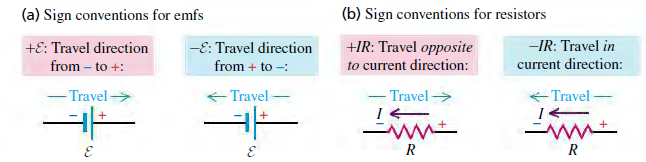
\includegraphics[width=0.9\textwidth]{DC_direction.png}} \\[-0.5em]
					Power & $\displaystyle P=V\!I=I^2\!R=\frac{V^2}{R}$ \\[-0.7em]
					Impedance & Impedance extends the concept of resistance to AC circuits, and possesses both magnitude and phase, unlike resistance, which has only magnitude. \\[-1em]
					Kirchoff's Loop Rule & The sum of voltage drops across all circuital elements (in a loop) is zero. \\[-1em]
					Kirchoff’s Junction Rule & At any point where there is a node formed by the junction of various current carrying branches, by current conservation, the sum of the currents going into the node must equal to the sum of the currents going out of the node. \\
					\bottomrule
				\end{tabular}
			\end{center}
			\subsubsection{Circuits containing non-ohmic devices with known V-I characteristics}
			\begin{center}
				\renewcommand{\arraystretch}{1.5}
				\begin{tabular}[h]{@{}l@{\hspace{1em}}p{9cm}@{}}
					\textbf{Semiconductors} & The resistance at a point is equal to the potential difference across the semiconductor divided by the current, \underline{\textbf{NOT necessarily the slope at the point}}
				\end{tabular}
			\end{center}
		\subsection{Magnetic field and Magnetic Forces}
			\begin{center}
				\renewcommand{\arraystretch}{2.3}
				\begin{tabular}[h]{@{}l@{\hspace{2em}}l@{}}
					\toprule
					Magnetic Force (f. wire) & $\bvec{F} = I \bvec{L}\times\bvec{B}$ \\
					Lorentz Force (f. moving point charge) & $\bvec{F} = q\left(\bvec{E} + \bvec{v}\times\bvec{B}\right)$ \\
					Biot-Savart Law {\small (f. wire)} & $\displaystyle \dif \bvec{B} = \frac{\mu_0 I}{4\pi} \frac{\dif \bvec{l}\times\bvec{r}}{|r|^3}$ \\
					Biot-Savart Law {\small (f. moving point charge)} & $\displaystyle \dif \bvec{B} = \frac{\mu_0 q}{4\pi} \frac{ \bvec{v}\times\bvec{r}}{|r|^3}$ \\
					Magnetic Dipole Moment & $\mu = N\bvec{I}\times\!\bvec{A}$\\
					Ampere’s Law & $\displaystyle \oint \bvec{B}\cdot \dif \bvec{l}= \mu_0I$\\[0.5em]
					\bottomrule
				\end{tabular}
			\end{center}
			
		\subsection{Electromagnetic induction and inductance}
			\begin{center}
				\renewcommand{\arraystretch}{2.3}
				\begin{tabular}[h]{@{}l@{\hspace{2em}}l@{}}
					\toprule
					Magnetic Flux & $\phi=\bvec{B}\cdot\!\bvec{A}$\\
					Faraday’s Law & $\varepsilon=-N\dod{\phi}{t}$\\[-1em]
					Lenz’s Law & $\hspace{2em}\uparrow$ accounts for negative sign\\
					Inductance & $V = L \dod{I}{t}$ \\[0.5em]
					\bottomrule
				\end{tabular}
			\end{center}
			\subsubsection{Self-Inductance}
				Consider a circuit consisting of a switch, power source and wires.
				
				Initially, current flows in the wire. When the switch is turned off, the current in the wire does not instantaneously drop to zero but slowly falls to zero. According to Faraday’s Law, this effect results in the induction of a magnetic field to oppose this change. This induced magnetic field is in the opposite direction of the magnetic field of the original current. This property of the loop in which its own magnetic field opposes any change in current is called self-inductance.
				
				\begin{equation*}
					\varepsilon_{\text{back}}=-L\dod{I}{t} \text{~~~~~~~~~where~~} L = \frac{N\phi}{I}
				\end{equation*}
			\pagebreak
			\subsubsection{Mutual Inductance}
				Consider two coils placed near to each other. 
				
				Suddenly, a current flows in the first coil (with $N$ turns and current $I_{\!A}$) which gives rise to a magnetic field. Some of the magnetic field lines through coil $A$ will also pass through coil $B$. This results in an increase in magnetic flux linkage through coil $B$. By Faraday’s Law, an induced emf occurs in coil $B$.
				\begin{equation*}
					N_{\!B}\dod{\phi_B}{t} = M\dod{I_{\!A}}{t} \text{~~~~~~~~~where~~} M=\frac{N_{\!B}\phi}{I_{\!A}}
					\vspace{-0.5em}
				\end{equation*}
	% \pagebreak?
	\section{Thermodynamics}
		\subsection{Laws of Thermodynamics and Absolute Temperature}
			\vspace{-0.5em}
			\begin{center}
				\renewcommand{\arraystretch}{1.2}
				\begin{tabular}{@{} l p{13cm} @{}}
					\toprule
					0\textsuperscript{th} & If two systems are in thermal equilibrium with a third system, they are in thermal equilibrium with each other. \\
					1\textsuperscript{st} & Increase in internal energy of system is sum of heat absorbed by system and work done on system. $$\Delta U = Q + W_{on}$$ \vspace*{-\baselineskip} \\
					\bottomrule
				\end{tabular}
			\end{center}
			 Absolute temperature (unit: Kelvin) is defined with reference to absolute zero. At absolute zero, particles have zero vibrational motion. For reference,
			 \begin{equation*}
				 \Delta \SI{1}{\degreeCelsius} = \Delta \SI{1}{\K} \text{~~and~~} \SI{0}{\degreeCelsius} = \SI{273.15}{\K}
				 \vspace{-0.5em}
			 \end{equation*}
		\subsection{Kinetic theory of an ideal gas}
			\begin{multicols}{2}
				Ideal gas equation:
				\begin{equation*}
					PV=nRT = NkT
				\end{equation*}
				\columnbreak
				
				For a monatomic gas particle:
				\begin{align*}
					v_{\text{rms}} &= \sqrt{\frac{3kT}{m}} = \sqrt{\frac{3RT}{M_{\text{molar}}}} \\
					E_k &= \frac{3}{2}NkT = \frac{3}{2}nRT
				\end{align*}
			\end{multicols}
			\vspace{-1em}
			where:
			\begin{center}
				\renewcommand{\arraystretch}{1}
				\begin{tabular}{@{} llll @{}}
					\toprule
					$P$ & Pressure & $T$ & Absolute Temperature\\
					$V$ & Volume & $k$ & Boltzmann Constant \\
					$n$ & No. of moles of gases & $N$ & Number of particles\\
					$R$ & Ideal gas constant &$M_\text{molar}$& Molar mass of the gas (in $\SI{}{\kg\per\mole}$)\\
					\bottomrule
				\end{tabular}
			\end{center}
			\vfill
			\textbf{Note:} $\SI{1}{\mole} = \SI{6.023e23}{}$ particles. This number is called the Avogadro’s number $N_{\!A}$.
			
			\textbf{Note:} We usually measure $M_\text{molar}$ in $\SI{}{\gram\per\mole}$. In this unit, it is numerically equal to the atomic mass of a gas particle/molecule.
		\subsection{Thermal properties of Materials}
			\begin{center}
				\renewcommand{\arraystretch}{1.2}
				\begin{tabular}{@{} l l @{}}
					\toprule
					Heat Capacity $c$ & $Q = mc\Delta\theta$ \\
					Latent Heat $Q$ & $Q = mL$ where $L$ is the process's \textit{specific latent heat} \\
					\bottomrule
				\end{tabular}
			\end{center}
			\vspace{\parskip}
			Latent heat is thermal energy released or absorbed, by a body or a thermodynamic system, during a constant-temperature process (e.g. boiling).
			
			\textbf{Note:} Heat capacity is different for different materials at different states. You will mostly be using the specific heat capacity $c$ of an object, and not $C = mc$, the heat capacity of the object.
			
			\textbf{Note:} $Q$ is heat energy in joules.
			
			\subsubsection{Thermal Conductivity}
				In an isotropic medium the thermal conductivity is the parameter $k$ in the Fourier expression for the heat flux $\bvec{q} = -k\bvec{\nabla}T$, where $\bvec{q}$ is heat flux (amount of heat flowing per second and per unit area), and $\bvec{\nabla}T$ the temperature gradient.
				
				In a one-dimensional case, it reduces to:
				\begin{equation*}
					H=-kA\dod{T}{x}
					\vspace{-0.5em}
				\end{equation*}
				where $\displaystyle q = \frac{H}{A} \implies H = qA = \dod{Q}{t}$. 
				
				$H$ is thus \textbf{the amount of heat flowing per second through a surface} with area $A$.
				
				If the temperature difference is small, $k$ can be taken as constant. The equation thus reduces to:
				\begin{equation*}
					H=kA{\frac {T_{\text{H}}-T_{\text{L}}}{L}}
				\end{equation*}
			\subsubsection{Thermal Expansion}
			\begin{center}
				\renewcommand{\arraystretch}{1.2}
				\begin{tabular}{@{} ccc @{}}
					\toprule
					Linear Expansion & Area Expansion & Volume Expansion \\[0.5em]
					$\displaystyle \frac{\Delta L}{L_0} = \alpha \Delta T$ & $\displaystyle \frac{\Delta A}{A_0} = 2\alpha \Delta T$ & $\displaystyle \frac{\Delta V}{V_0} = 3\alpha \Delta T$ \\[0.5em]
					\bottomrule
				\end{tabular}
			\end{center}
		\pagebreak
		\subsection{Thermodynamic Processes}
			The 1\textsuperscript{st} Law of Thermodynamics is relevant to many Thermodynamics Processes.
			
			For any process, the work done by an expanding gas $W_{\text{by}}=-W_{\text{on}}$ is given by:
			\begin{equation*}
				W_{\text{by}}=P\Delta V \impliedby \dif W_{\text{by}} = \int\! P \dif V
				\vspace{-1em}
			\end{equation*}
			
			We assume, for the following P-V graphs, that the arrow points towards the positive-$V$ direction. 
			\begin{center}
				\renewcommand{\arraystretch}{1.2}
				\begin{tabular}{@{} l l l @{}}
					\toprule
					Isobaric & Constant Pressure  & $W_{on} < 0 ~,~~ \Delta U > 0$\\
					Isochoric & Constant Volume & $W_{on} = 0 ~,~~ \Delta U > 0$\\
					Isothermal & Constant Temperature & $W_{on} < 0 ~,~~ \Delta U = 0$\\
					Adiabatic & Thermally Insulated & $W_{on} < 0 ~,~~ Q = 0$\\
					Cyclic & Start and end at the same state & $\Delta U = 0$\\
					\bottomrule
				\end{tabular}
			\end{center}
			\vspace{\parskip}		
			Work is done \underline{\textbf{by the gas}} when \underline{\textbf{expanding}}; \\
			Work is done \underline{\textbf{on the gas}} when \underline{\textbf{contracting}}.
			
			The internal energy $U$ is the microscopic kinetic energy $E_k$ of the particles. For a monatomic particle $$U=\frac{3}{2}nRT$$
			\subsubsection{Thermodynamic efficiency}
			The thermal efficiency $\eta_\text{th}$ is given by:
			\begin{equation*}
				\eta _{\text{th}}\equiv {\frac {W_{out}}{Q_{in}}}={\frac {{Q_{in}}-Q_{out}}{Q_{in}}}=1-{\frac {Q_{out}}{Q_{in}}}
			\end{equation*}
			
\end{document}